%-------------------------------------------------------------------------------
%-------------------------------------------------------------------------------
%-------------------------------------------------------------------------------
\chapter{Listes : 2}
%-------------------------------------------------------------------------------
%-------------------------------------------------------------------------------
\thispagestyle{empty}
%-------------------------------------------------------------------------------
%-------------------------------------------------------------------------------
{\sf Dans ce T.P. nous allons utiliser construire ou modifier des listes. Dans le cas de constructions de listes, les énoncés ne considèrent que des listes de taille fixées à l'avance. Les cas plus général de listes sans connaître à l'avance la taille sera vu dans un autre T.P. 

Une liste de taille $n$ pourra être construite selon le motif
\begin{lstlisting}
def fonction(...):
    ...
    L = [0]*n
    for i in range(n):
        ...
        L[i] = ...
    return L
\end{lstlisting}
}
%-------------------------------------------------------------------------------
%-------------------------------------------------------------------------------
%-------------------------------------------------------------------------------
\section{Fonctions mathématiques} 
%-------------------------------------------------------------------------------
%-------------------------------------------------------------------------------
%-------------------------------------------------------------------------------
\begin{Exercise}[title = Carrés]
\it Écrire une fonction \type{carre(liste)} qui renvoie la liste de même taille que la liste passée en paramètre et dont les éléments sont les carrés de éléments de celle-ci.
\end{Exercise}
%-------------------------------------------------------------------------------
\begin{Answer}
\begin{lstlisting}
def carres(liste):
    n = len(liste)
    L = [0]*n
    for i in range(n):
        L[i] = liste[i]**2
    return L
\end{lstlisting}
\end{Answer}
%-------------------------------------------------------------------------------
%-------------------------------------------------------------------------------

\medskip

La fonction ci-dessus peut se généraliser. 

Une fonction peut recevoir une autre fonction comme paramètre.
%-------------------------------------------------------------------------------
%-------------------------------------------------------------------------------
\begin{Exercise}[title = Image d'une liste par une fonction]
\it Écrire une fonction \type{appliquer(f, liste)} qui renvoie la liste des valeurs $f(x)$ pour les éléments $x$ de la liste.
\end{Exercise}
%-------------------------------------------------------------------------------
\begin{Answer}
\begin{lstlisting}
def appliquer(f, liste):
    n = len(liste)
    L = [0]*n
    for i in range(n):
        L[i] = f(liste[i])
    return L
\end{lstlisting}
\end{Answer}
%-------------------------------------------------------------------------------
%-------------------------------------------------------------------------------
Par exemple si on définitions
\begin{lstlisting}
def harmo(x):
    return (x+4)/(x+1)
\end{lstlisting}
\type{appliquer(harmo, [0, 1, 2, 3, 4])} renverra \type{[4.0, 2.5, 2.0, 1.75, 1.6]}.
\medskip

On peut écrire le résultat de \type{appliquer(f, liste)} plus simplement avec 
\begin{lstlisting}
[f(x) for x in liste]
\end{lstlisting}
%-------------------------------------------------------------------------------
%-------------------------------------------------------------------------------
\subsection{Graphe d'une fonction} 
%-------------------------------------------------------------------------------
%-------------------------------------------------------------------------------
\begin{Exercise}\it
Écrire une fonction \type{listeX(a, b, n)} qui calcule une liste de longueur $n$ dont les valeurs sont équiréparties entre $a$ et $b$.
\end{Exercise}
%-------------------------------------------------------------------------------
\begin{Answer}
\begin{lstlisting}
def listeX(a, b, n):
    pas = (b-a)/(n-1)
    X = [0]*n
    for k in range(n):
        X[k] = a + k*pas 
    return X
\end{lstlisting}
\end{Answer}
%-------------------------------------------------------------------------------
%-------------------------------------------------------------------------------
\smallskip
\type{listeT(1, 3, 5)} doit renvoyer \type{[1.0, 1.5, 2.0, 2.5, 3.0]}.

On remarquera que l'écart entre deux points consécutifs est $\frac{b-a}{n-1}$, dans la liste renvoyée le terme d'indice i est donc
$a + i\frac{b-a}{n-1}$. Il est recommandé de stocker la valeur $\frac{b-a}{n-1}$ dans une variable.

\bigskip

On peut maintenant représenter une fonction sur un intervalle $[a;b]$.

\begin{enumerate}
\item On définit la fonction python correspondant à la fonction à étudier.

On pourra utiliser le module \type{math} pour obtenir les fonctions mathématiques usuelles.
\begin{lstlisting}
import math as m
\end{lstlisting}
On pourra utiliser \type{m.cos}, \type{m.exp}, \type{m.pi}, \dots

\item On crée une liste d'abscisse avec \type{X = listeX(a, b, 500)}\footnote{500 points suffisent dans la plupart des cas.}.
\item On crée la liste des ordonnées avec \type{Y = appliquer(f, X)}
\item On trace le graphe, il faudra avoir chargé le sous-module \type{pyplot}.
\begin{lstlisting}
import matplotlib.pyplot as plt
...    
plt.plot(X, Y)
plt.show()
\end{lstlisting}
\end{enumerate}
%-------------------------------------------------------------------------------
%-------------------------------------------------------------------------------
\begin{Exercise}\it
Tracer le graphe de $f$ : $x\mapsto e^{-x}\cos(\pi x)$ sur $[0:5].$
\end{Exercise}
%-------------------------------------------------------------------------------
\begin{Answer}
\begin{lstlisting}
def f(x):
    return m.exp(-x)*m/cos(m.pi*x)
    
X = listeX(0, 5, 500)
Y = appliquer(f, X)
plt.plot(X, Y)
plt.show()
\end{lstlisting}
\end{Answer}
%-------------------------------------------------------------------------------
%-------------------------------------------------------------------------------
\medskip

Quand on veut tracer les graphes de plusieurs fonctions, on peut les référencer en ajoutant la variable optionnelle \type{label} qui qui doit être une chaîne de caractère, elle sera affichée par \type{plt.legend()}.
\begin{lstlisting}
X = listeX(-3, 5, 500)
Y1 = appliquer(m.cos, X)
Y2 = appliquer(m.sin, X)
plt.plot(X, Y1, label="cosinus")
plt.plot(X, Y2, label="sinus")
plt.legend()
plt.show()
\end{lstlisting}
%-------------------------------------------------------------------------------
%-------------------------------------------------------------------------------
\begin{center}
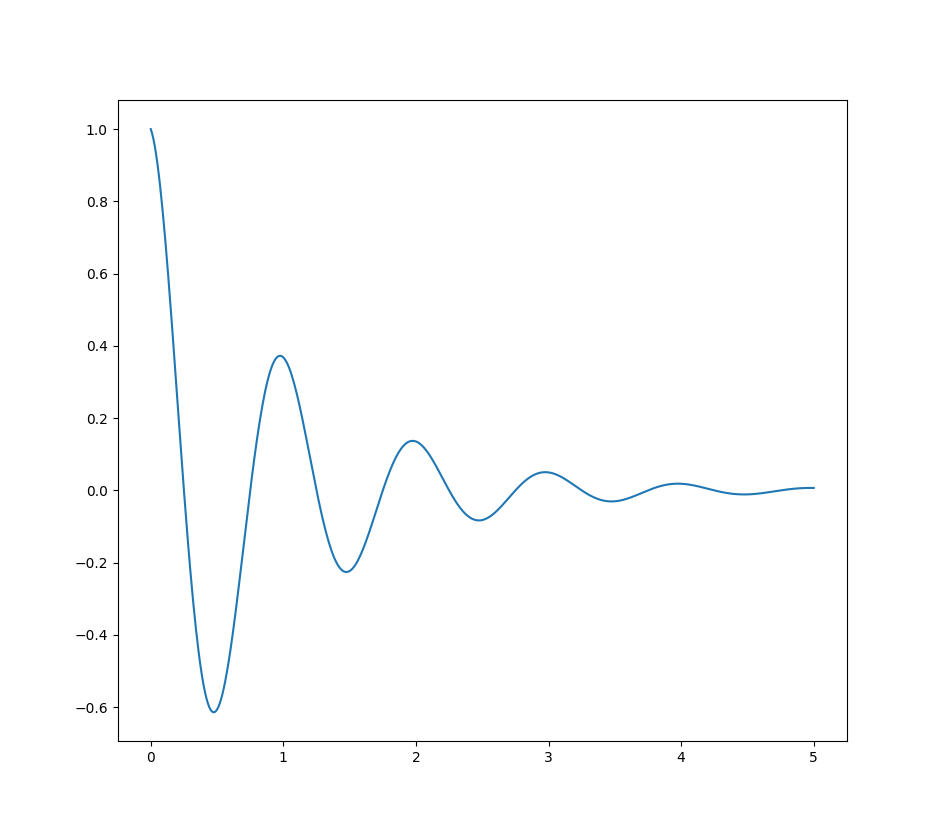
\includegraphics[width=0.49\linewidth]{TP07_exp.png}
\hfill
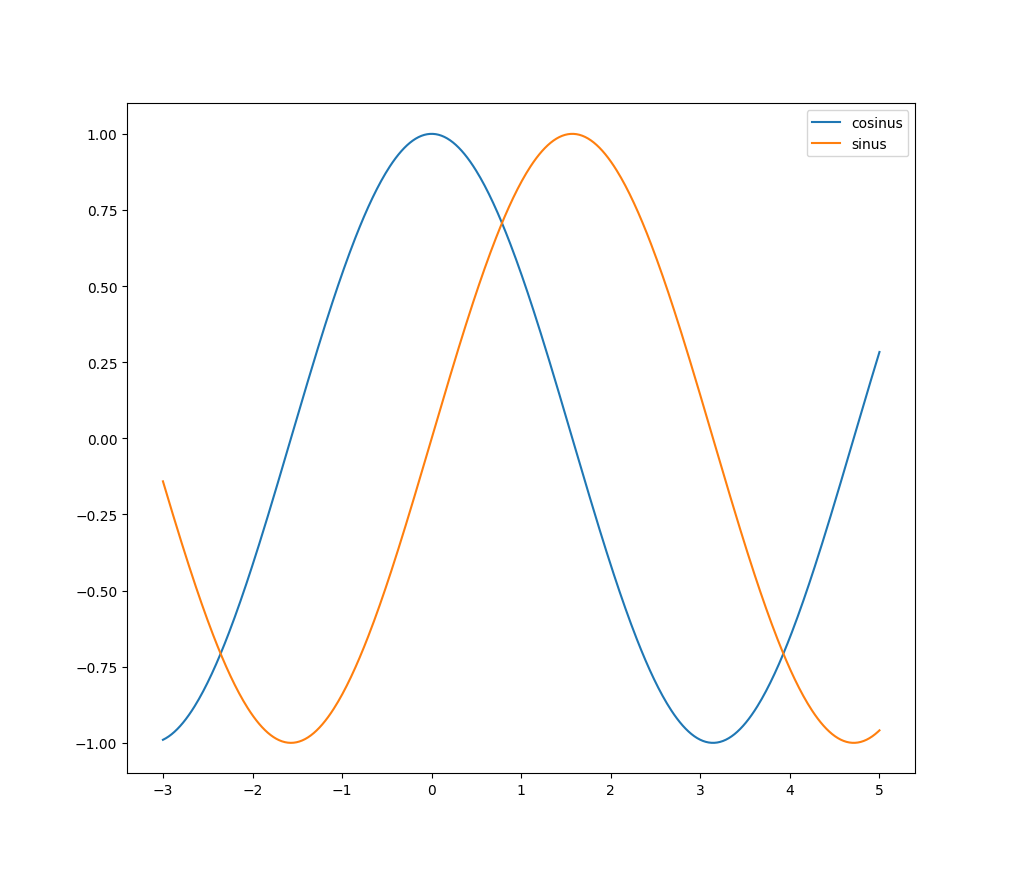
\includegraphics[width=0.49\linewidth]{TP07_cos_sin.png} 
\end{center}
%-------------------------------------------------------------------------------
%-------------------------------------------------------------------------------
%-------------------------------------------------------------------------------
\section{Tirages aléatoires  } 
%-------------------------------------------------------------------------------
%-------------------------------------------------------------------------------
%-------------------------------------------------------------------------------
Dans le module \type{random}, la fonction à deux variables entières \type{randint(a, b)} renvoie un entier au hasard compris entre $a$ et $b$ avec $a$ et $b$ compris.
%-------------------------------------------------------------------------------
\begin{lstlisting}
from random import randint
print(randint(4, 12))
\end{lstlisting}
%-------------------------------------------------------------------------------
On obtient un entier différent à chaque appel appartenant à $\{4, 5, \ldots, 12\}$.
%-------------------------------------------------------------------------------
%-------------------------------------------------------------------------------
\begin{Exercise}[title= Tirages de dés]\it
Écrire une fonction \type{tiragesDe(n)} qui renvoie une liste de taille $n$ dont les valeurs sont choisies aléatoirement entre 1 et 6.

Par exemple \type{tiragesDe(12)} peut renvoyer 
\type{[6, 5, 3, 3, 2, 2, 6, 4, 6, 5, 6, 1]}.
%-------------------------------------------------------------------------------
\end{Exercise}
%-------------------------------------------------------------------------------
\begin{Answer}
%-------------------------------------------------------------------------------
\begin{lstlisting}
from random import randint

def tiragesDe(n):
 	"""Entrée : un entier positif
 	   Sortie : la liste des tirages de n dés""" 
    resultat = [0]*n
    for i in range(n):
        resultat[i] = randint(1, 6)
    return resultat
\end{lstlisting}
%-------------------------------------------------------------------------------
\end{Answer}
%-------------------------------------------------------------------------------
%-------------------------------------------------------------------------------
\begin{Exercise}[title= Occurrences]\it
Écrire une fonction \type{occurrences(liste)} qui renvoie une liste de taille 6 dont les valeurs sont les nombres d’occurrences des entiers de 1 à 6 dans une liste ne contenant que des entiers entre 1 et 6. Le terme d'indice $i$ de la liste ($0\le i < 6$) contiendra le nombre d’occurrences de $i+1$.
%-------------------------------------------------------------------------------
\end{Exercise}
%-------------------------------------------------------------------------------
\begin{Answer}
%-------------------------------------------------------------------------------
\begin{lstlisting}
def occurrences(liste):
 	"""Entrée : un entier positif
 	   Sortie : la liste de la distribution des valeurs
 	            d'une liste d'entiers de 1 à 6""" 
    n = len(liste)
    resultat = [0]*6
    for i in range(n):
        k = liste[i] - 1
        resultat[k] += 1
    return resultat
\end{lstlisting}
%-------------------------------------------------------------------------------
\end{Answer}
%-------------------------------------------------------------------------------
%-------------------------------------------------------------------------------

\medskip

\begin{minipage}[b]{0.55\textwidth}

On peut représenter le résultat par un histogramme.

\begin{enumerate}
\item On crée une liste de tirages : \type{T = tiragesDe(1200)}.
\item On répartit les tirages : \type{occ = occurrences(X)}.
\item On crée la liste des valeurs comptées : \type{X = [1, 2, 3, 4, 5, 6]}
\item On trace le graphe en barres
\begin{lstlisting}
plt.bar(X, occ)
plt.show()
\end{lstlisting}
\end{enumerate}
\end{minipage}
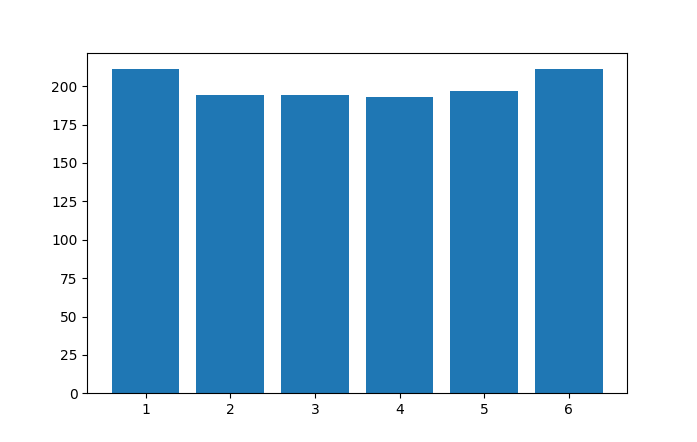
\includegraphics[width=0.50\linewidth]{TP07_des.png} 
%-------------------------------------------------------------------------------
%-------------------------------------------------------------------------------
%-------------------------------------------------------------------------------
\section{Suites} 
%-------------------------------------------------------------------------------
%-------------------------------------------------------------------------------
%-------------------------------------------------------------------------------
On a déjà vu la suite des nombres de Fibonacci ils sont définis par

\begin{center}
$F_0 = 0,\ F_1 = 1 \hbox{ et }F_{n+2} = F_{n+1} + F_n \hbox{ pour }n\in {\mathbb N}$
\end{center}

%-------------------------------------------------------------------------------
%-------------------------------------------------------------------------------
\begin{Exercise}[title=Nombres de Fibonacci]\it
Écrire une fonction \type{liste\_fibo(n)} qui renvoie la liste formée des $n+1$ premiers nombres de Fibonacci, de $F_0$ à $F_n$. On notera qu'on doit renvoyer $n+1$ valeurs.
\end{Exercise}
%-------------------------------------------------------------------------------
\begin{Answer}
%-------------------------------------------------------------------------------
\begin{lstlisting}
def liste_fibo(n)
    F = [0]*(n+1)
    F[1] = 1 # F[0] vaut déjà 0
    for k in range(n-1): # 
        F[k+2] = F[k+1] + F[k] 
    return F
\end{lstlisting}
%-------------------------------------------------------------------------------
\end{Answer}
%-------------------------------------------------------------------------------
%-------------------------------------------------------------------------------

\medskip

Les nombres de Catalan sont des entiers qui apparaissent dans de nombreux problèmes de dénombrement.
Une de leurs définitions est la récurrence :

\begin{center}
$\displaystyle C_0 = 1 \hbox{ et }C_{n+1}=\sum_{i=0}^n C_iC_{n-i}\hbox{ pour }n\in {\mathbb N}$
\end{center}

%-------------------------------------------------------------------------------
%-------------------------------------------------------------------------------
\begin{Exercise}[title=Nombres de Catalan]\it 
Écrire une fonction \type{catalan(n)} qui renvoie la liste formée des nombres de Catalan de $C_0$ à $C_n$.

\end{Exercise}
%-------------------------------------------------------------------------------
\begin{Answer}
%-------------------------------------------------------------------------------
\begin{lstlisting}
def catalan(n):
 	"""Entrée : un entier positif
 	   Sortie : la liste des nombres de catalan de C(0) à C(n)"""
    C = [0]*(n+1)
    C[0] = 1
    for k in range(n): # On calcule C(k+1)
        somme = 0
        for i in range(k+1): # i de 0 à k 
            somme = somme + C[i]*C[k-i] 
        C[k+1] = somme 
    return C
\end{lstlisting}
%-------------------------------------------------------------------------------
\end{Answer}
%-------------------------------------------------------------------------------
%-------------------------------------------------------------------------------
\medskip

On rappelle qu'on a $\displaystyle  \binom n{k+1} = \frac{n-k}{k+1} \binom nk$.
%-------------------------------------------------------------------------------
%-------------------------------------------------------------------------------
\begin{Exercise}[title= Coefficients binomiaux, bis]
Écrire une fonction \type{liste_binom(n)} qui renvoie la liste des $\binom nk$ pour $0\le k \le n$.
\end{Exercise}
%-------------------------------------------------------------------------------
\begin{Answer} 
\begin{lstlisting}
def liste_binom(n):
    bin = [0]*n
    bin[0] = 1
    for k in range(n):
        bin[k+1 = bin[k]*(n-k)//(k+1)
    return bin
\end{lstlisting}
\end{Answer}
%-------------------------------------------------------------------------------


%-------------------------------------------------------------------------------
%-------------------------------------------------------------------------------
\begin{Exercise}[title= Retourner une liste]
%-------------------------------------------------------------------------------
\begin{enumerate}
\item Écrire un programme qui renvoie une liste passée en paramètre dans l'ordre inverse.
\item Écrire un programme qui retourne une liste "en place".
\end{enumerate}
%-------------------------------------------------------------------------------
\end{Exercise}
%-------------------------------------------------------------------------------
\begin{Answer}
\begin{enumerate}
 \item On peut écrire la liste terme-à-terme en lisant la liste initiale à l'envers.
%-------------------------------------------------------------------------------
\begin{lstlisting}
def listeInverse(liste):
 	"""Entrée : une liste
	   Sortie : une liste avec les termes inversés"""
    n = len(liste)
    etsil = [0]*n # liste à l'envers :)
	  for i in range(n): 
	      etsil[i] = liste[n - 1- i]
	  return etsil
\end{lstlisting}
%-------------------------------------------------------------------------------
\item Ce n'est pas la même question, on modifie la liste "en place".

On utilise la fonction \type{echange} de ce chapitre.
%-------------------------------------------------------------------------------
\begin{lstlisting}
def retourner(liste):
  """Entrée : une liste
      Sortie : la liste est retournée"""
  n = len(liste)
  for i in range(n//2): 
      echange(liste,i,n-1-i)
\end{lstlisting}
%-------------------------------------------------------------------------------
Il ne faut pas faire des échanges du début jusqu'à la fin car sinon on remet en place les éléments retournés.
On doit échanger les éléments d'indice 0 à $p-1$ si $n=2p$ ou $n=2p+1$ (le milieu reste en place).
\end{enumerate}
%-------------------------------------------------------------------------------
\end{Answer}


%-------------------------------------------------------------------------------
%-------------------------------------------------------------------------------
\begin{Exercise}[title= Lissage d'une liste]
%-------------------------------------------------------------------------------
Lorsque l'on traite des données acquises lors d'une expérimentation, les résultats sont souvent perturbés par des fluctuations, du bruit. 

\begin{minipage}[b]{0.55\textwidth}
Pour éliminer ce bruit, une technique possible est de lisser les valeurs en les moyennant.

Dans la pratique, si les valeurs de la liste sont $a_0, a_1, \ldots, a_{n-1}$, on crée une liste de taille $n$ et on affecte avec les valeurs $b_k$ définies par
\[
\left\{\begin{matrix} b_0 = \frac{a_0+a_1}2\quad 
b_{n-1} = \frac{a_{n-2}+a_{n-1}}2\\
 b_k = \frac{a_{k-1}+2a_k+a_{k+1}}4
 \text{ pour }1\le k \le n-2
\end{matrix}
\right.
\]

Dans le graphe ci-contre on a calculé (voir ci-dessous) une liste et on a appliqué le lissage puis on a répété 10 fois le lissage pour obtenir la liste représentée en bas. 
\end{minipage}
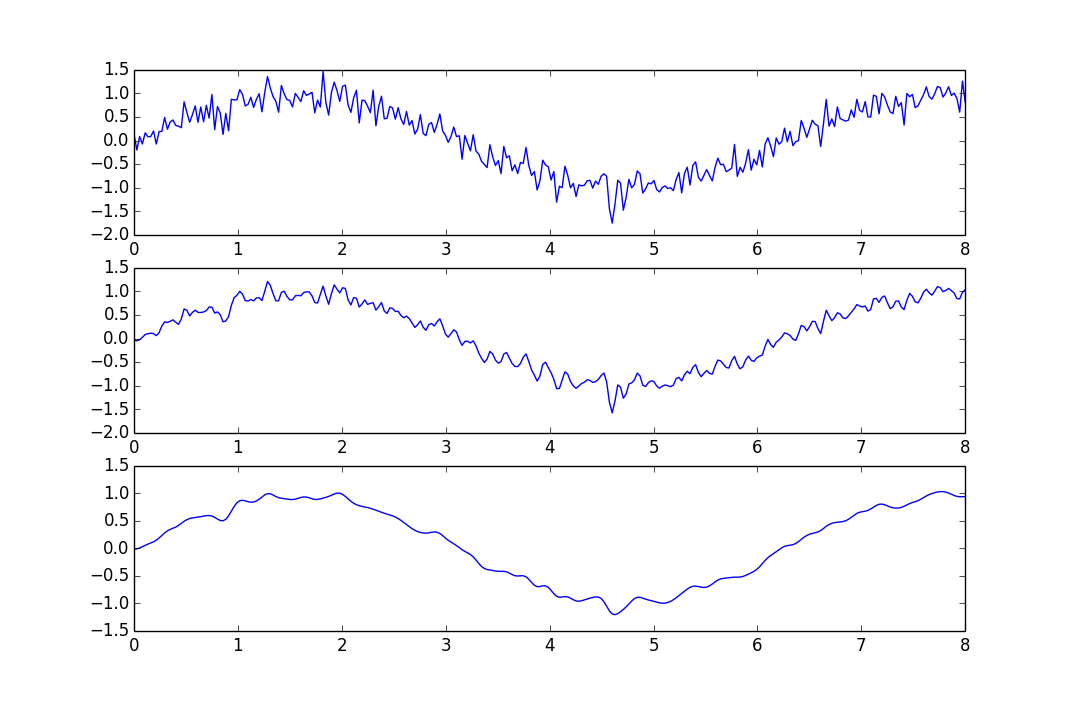
\includegraphics[scale=0.33]{03_lissage.png} 

\begin{lstlisting}
l = [math.sin(i/30)+random.normalvariate(0, 0.1) 
                             for i in range(250)]
\end{lstlisting}
Écrire une fonction \type{lissage(liste)}
%-------------------------------------------------------------------------------
%-------------------------------------------------------------------------------
\end{Exercise}
%-------------------------------------------------------------------------------
\begin{Answer}
\begin{lstlisting}
def lissage(liste):
    n = len(liste)
    lisse = [0]*n
    lisse[0] = (liste[0] + liste[1])/2
    for i in range(1, n-1):
        lisse[i] = (liste[i-1] + 2*liste[i] + liste[i+1])/4
    lisse[n-1] = (liste[n-2] + liste[n-1])/2
    return lisse
\end{lstlisting}
%-------------------------------------------------------------------------------
\newpage
\end{Answer}
\begin{Exercise}[title= Insertion dans une liste]
%-------------------------------------------------------------------------------
Écrire une fonction \type{inserer(x,i,liste)} qui renvoie une nouvelle liste où, à partir de \type{liste}, on a inséré l'élément \type{x} à la position \type{i} et décalé les suivants vers la droite.
\end{Exercise}
%-------------------------------------------------------------------------------
\begin{Answer}
le plus simple est d'utiliser les extractions.

On rappelle que \type{liste[:i]+liste[i:]} reconstitue la liste.
%-------------------------------------------------------------------------------
\begin{lstlisting}
def inserer(x,i,liste):
    """Entrée : un élément x, un entier i et une liste
                on doit avoir 0 <= i <= len(liste)
       Sortie : la liste avec x inséré à la position i"""
    return liste[:i]+[x]+liste[i:]
\end{lstlisting}
\end{Answer}
%-------------------------------------------------------------------------------
%-------------------------------------------------------------------------------
\begin{Exercise}[title= Suppression d'une position]
 Écrire une fonction \type{supprimer\_place(i, liste)} qui renvoie une nouvelle liste où, à partir de \type{liste}, on a supprimé l'élément d'indice \type{i}. Les éléments suivants doivent être décalés vers la gauche.
\end{Exercise}
%-------------------------------------------------------------------------------
\begin{Answer}
\begin{lstlisting}
def supprimer_place(i,liste):
    """Entrée : un entier i et une liste, 0 <= i < len(liste)
       Sortie : la liste moins le i-ième élément"""
    return liste[:i]+liste[i+1:]
\end{lstlisting}
\end{Answer}
%-------------------------------------------------------------------------------
%-------------------------------------------------------------------------------
\begin{Exercise}[title=Maximum]
Écrire une fonction qui calcule le maximum des termes d'une liste.
\end{Exercise}
%-------------------------------------------------------------------------------
\begin{Answer}
%-------------------------------------------------------------------------------
\begin{lstlisting}
def maxListe(liste):
	  """Entrée : une liste non vide
	     Sortie : la valeur du maximum de la liste"""
  maximum = liste[0] # Un maximum provisoire
  n = len(liste)
  for i in range(n):
      if maximum < liste[i]:
          maximum = liste[i]
  return maximum
\end{lstlisting}
%-------------------------------------------------------------------------------
On compare inutilement le premier terme avec lui-même pour $i=0$. On pouvait écrire \type{for i in range(1,n)}, dans le cas $n=1$ aucune itération n'est calculée.

\medskip

On pouvait aussi se passer de l'indice :
%-------------------------------------------------------------------------------
\begin{lstlisting}
def maxListe(liste):
 	"""Entrée : une liste non vide
	     Sortie : la valeur du maximum de la liste"""
  maximum = liste[0] # Un maximum provisoire
  for x in liste:
      if maximum < x:
          maximum = x
  return maximum
\end{lstlisting}
%-------------------------------------------------------------------------------
\end{Answer}
%-------------------------------------------------------------------------------
%-------------------------------------------------------------------------------
\begin{Exercise}[title=Positivité 2]
On reprend les questions de l'exercice \ref{exo:pos1} mais on demande de cesser les tests des éléments de la liste dès que le résultat est certain.
%-------------------------------------------------------------------------------
\begin{enumerate}
    \item Écrire une fonction \type{tout\_positif(liste)} qui renvoie \type{True} ou \type{False} selon que tous les éléments de la liste sont positifs ou non.
    \item Écrire une fonction \type{existe\_positif(liste)} qui renvoie \type{True} s'il existe au moins un élément positif dans la liste et \type{False} sinon.
\end{enumerate}
%-------------------------------------------------------------------------------
\end{Exercise}
%-------------------------------------------------------------------------------
\begin{Answer}
%-------------------------------------------------------------------------------
\begin{enumerate}
\item Le résultat est certain si on a trouvé une valeur négative : dans ce cas la réponse est \type{False}. Si toute la boucle est parcourue sans sortie c'est que toutes les valeurs sont positives.
\begin{lstlisting}
def tout_positif(liste):
    """Entrée : une liste de nombre
       Sortie : True si tous les termes sont positifs
                False sinon"""
    for x in liste:
        if x < 0:
            return False
    return True
\end{lstlisting}
%-------------------------------------------------------------------------------
\item Ici le cas est symétrique, une valeur positive permet de conclure \type{True}
\begin{lstlisting}
def existe_positif(liste):
    """Entrée : une liste de nombre
       Sortie : True si au moins un terme est positif
                False sinon"""
    for x in liste:
        if x >= 0:
            return True
    return False
\end{lstlisting}
\end{enumerate}
%-------------------------------------------------------------------------------
\end{Answer}
%-------------------------------------------------------------------------------
%-------------------------------------------------------------------------------
\begin{Exercise}[title=Transformation de Cesàro]

La transformée de Cesàro\footnote{D'après le lemme de Cesàro, si une suite converge vers $\ell$,  sa transformée de Cesàro converge vers $\ell$ aussi.} d'une suite $(u_n)$ est la suite $(v_n)$ définie par $\displaystyle v_n= \frac 1{n +1}\sum_{k=0}^n u_k$. 



 Écrire une fonction \type{cesaro(liste)} qui renvoie les $n$ premiers termes de la transformée de Cesàro d'une suite donnée par les éléments de la liste de longueur $n$.
%-------------------------------------------------------------------------------
\end{Exercise}
%-------------------------------------------------------------------------------
\begin{Answer}
\begin{lstlisting}
def cesaro(liste):
    """Entrée : une liste de nombre
       Sortie : la suite transformée de Cesaro"""
    n = len(liste)
    ces = [0]*n
    somme = 0
    for k in range(n):
        somme = somme + liste[k]
        ces[k] = somme/(k+1)
    return ces
\end{lstlisting}
%-------------------------------------------------------------------------------
\end{Answer}
%-------------------------------------------------------------------------------
%-------------------------------------------------------------------------------

La {\bf variance} d'une liste est définie par $\displaystyle \text{var}(X) =  \frac 1n \sum_{i=0}^n \bigl(\type{X[i]} -m_X\bigr)^2$ avec $m_X$ égal à la moyenne de la liste et $n = \type{len(X)}$.
%-------------------------------------------------------------------------------
%-------------------------------------------------------------------------------
\begin{Exercise}[title = Variance]
\it Écrire une fonction \type{var(X)} qui calcule la variance de la liste $X$.

On affectera la moyenne dans une variable avant la boucle pour éviter de répéter le même calcul.

\type{variance(Z0)} donne \type{6.558001189767997}
\end{Exercise}
%-------------------------------------------------------------------------------
\begin{Answer}
\begin{lstlisting}
def var(X):
    n = len(X)
    mX = moyenne(X)
    somme = 0
    for x in X:
        somme = somme + (x - mX)**2
    return somme/n
\end{lstlisting}
\end{Answer}
%-------------------------------------------------------------------------------
%-------------------------------------------------------------------------------
\bigskip

Si $X$ et $Y$ sont deux listes de même longueur, la {\bf covariance} de $X$ est $Y$ est 

$\displaystyle \text{cov}(X, Y) =  \frac 1n \sum_{i=0}^n \bigl(\type{X[i]} -m_X\bigr)\bigl(\type{Y[i]} -m_Y\bigr)$ avec $m_X$ égal à la moyenne de la liste $X$, $m_Y$ égal à la moyenne de la liste $Y$ et $n$ est la longueur commune de $X$ et de $Y$.

On pourra noter que $\text{var}(X) = \text{cov}(X, X)$
%-------------------------------------------------------------------------------
%-------------------------------------------------------------------------------
\begin{Exercise}[title = Covariance]
\it Écrire une fonction \type{cov(X, Y)} qui calcule la covariance des listes $X$ et $Y$.

Il sera nécessaire ici d'accéder aux éléments de \type{X} et \type{Y} par leurs indices.

\type{cov(T0, X0)} donne \type{-1.6044390243902438}
\end{Exercise}
%-------------------------------------------------------------------------------
\begin{Answer}
\begin{lstlisting}
def cov(X, Y):
    n = len(X)
    mX = moyenne(X)
    mY = moyenne(Y)
    somme = 0
    for i in range(n):
        somme = somme + (X[i] - mX)*(Y[i] - mY)
    return somme/n
\end{lstlisting}
\end{Answer}
%-------------------------------------------------------------------------------
%-------------------------------------------------------------------------------
\bigskip


On admet que, $X$ et $Y$ sont deux listes de même longueur, alors la {\bf droite de régression} approchant $Y$ par rapport à $X$ est la droite d'équation $y = ax+b$ avec $m_Y = a.m_X + b$ et $a.\text{var}(X)=\text{cov}(X, Y)$.
%-------------------------------------------------------------------------------
%-------------------------------------------------------------------------------
\begin{Exercise}[title = Droite de régression]
\it Écrire une fonction \type{regression(X, Y)} qui calcule les coefficients$a$ et $b$ de la droite de régression de $X$ à $Y$.

\type{regression(X0, Y0)} donne \type{(2.2937900415993773, 1.7193194828375322)}
\end{Exercise}
%-------------------------------------------------------------------------------
\begin{Answer}
\begin{lstlisting}
def regression(X, Y):
    a = cov(X, Y)/var(X)
    b = moyenne(Y) - a*moyenne(X)
    return a, b
\end{lstlisting}
\end{Answer}
%-------------------------------------------------------------------------------
%-------------------------------------------------------------------------------
\subsection{Premiers graphes} 
%-------------------------------------------------------------------------------
%-------------------------------------------------------------------------------
Le module \type{matplotlib} permet de tracer des représentations de valeurs, c'est particulièrement utile dans le cas de listes. Nous utiliserons la sous-bibliothèque \type{pyplot} que l'on simplifiera par \type{plt}.
\begin{lstlisting}
import matplotlib.pyplot as plt
\end{lstlisting}

Il existe deux modes de tracé.
\begin{enumerate}
    \item Le mode standard construit les graphismes {\bf sans les afficher}, ils sont enrichis pas-à-pas. Quand toutes les instructions sont écrites, on demande l'affichage par \type{plt.show()} ; une fenêtre avec les graphismes apparaît et il faut la refermer pour continuer à utiliser Python. Nous utiliserons ce mode.
    \item Le mode interactif permet l'affichage de chaque commande en temps réel, sans monopoliser Python. Le principal inconvénient est que les graphismes deviennent vite surchargés, il faut régulièrement les effacer (\type{plt.clf()}). 
    \item On passe en mode interactif avec \type{plt.ion}, on en sort avec \type{plt.ioff}.
\end{enumerate}

\medskip

La fonction principale est \type{plt.plot}. Elle admet 2 utilisations.
\begin{enumerate}
    \item \type{plt.plot(X)} où \type{X} est une liste, relie les points de coordonnées \type{(i, X[i])} par des segments de droite, elle présente les valeurs de \type{X} dans l'ordre de la liste.
    \item \type{plt.plot(X, Y)} où \type{X} et \type{Y} sont deux listes {\bf de même longueur} relie les points de coordonnées \type{(X[i], Y[i])} par des segments de droite, elle présente les évolutions des les valeurs de \type{Y} en fonction de celles de \type{X}.
    \item Quand la liste n'est pas triée dans l'ordre croissant, la représentation ci-dessus n'est pas très signifiante. Parmi les nombreuses options de tracé, il existe la possibilité de représenter simplement les points sans tracer les segment avec un paramètre supplémentaire \type{'o'}, 
\end{enumerate}
%-------------------------------------------------------------------------------
\begin{center}
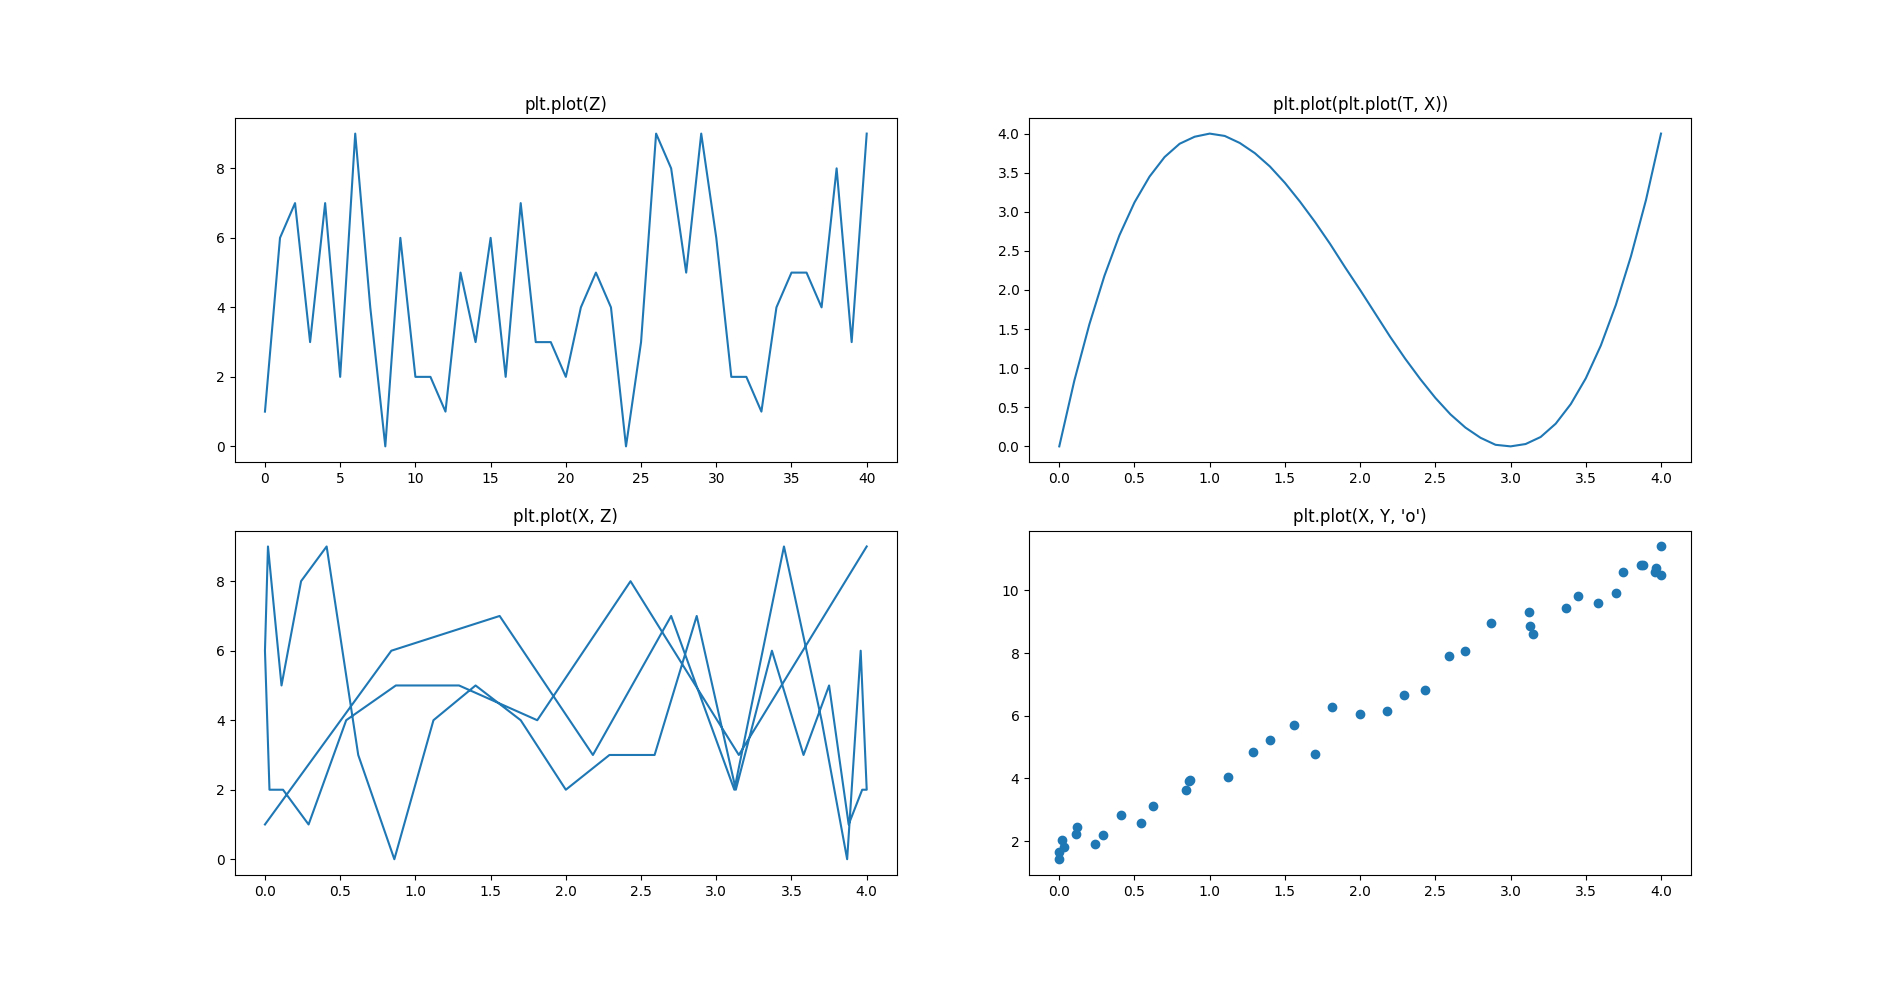
\includegraphics[width=1\linewidth]{TP06_plt.png} 
\end{center}
%-------------------------------------------------------------------------------

\vskip -1cm

On peut tracer plusieurs représentations (\type{plt.plot}) sur un même graphe.
%-------------------------------------------------------------------------------
%-------------------------------------------------------------------------------
\begin{Exercise}[title=Tracé de la droite de régression]
\it Après avoir calculé les coefficients ($a$ et $b$) de la droite de régression approchant \type{Y0} en fonction de \type{X0}, représenter sur un même graphe les points de coordonnées \type{(X0[i], Y0[i])} et la droite de régression. Pour tracer une droite d'équation $y = ax + b$ sur $[\alpha, \beta]$, on pourra tracer le segment entre les points $(\alpha, a.\alpha + b)$ et $(\beta, a.\beta + b)$.
\end{Exercise}
%-------------------------------------------------------------------------------
\begin{Answer}
\begin{lstlisting}
a, b = regression(X0, Y0)
c = a*4 + b
plt.plot(X0, Y0, 'o')
plt.plot([0, 4], [b, c])
plt.show()
\end{lstlisting}
%-------------------------------------------------------------------------------
\begin{center}
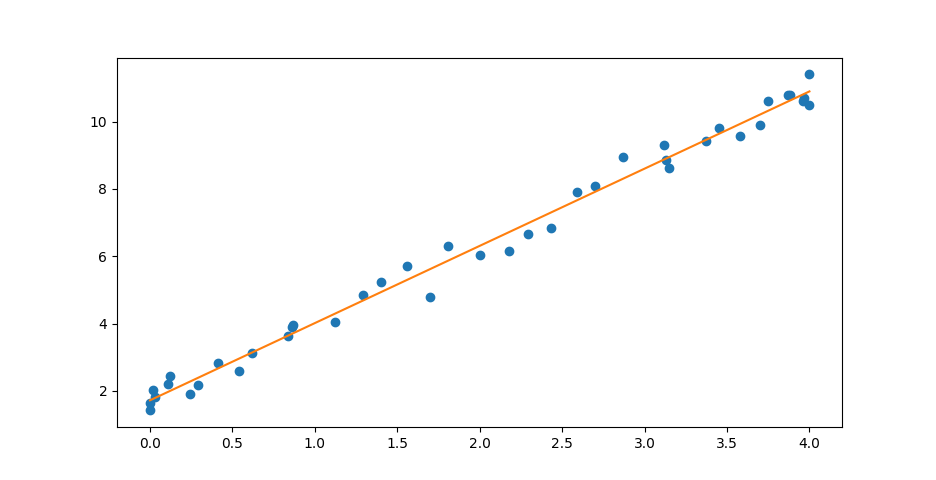
\includegraphics[width=1\linewidth]{TP06_ex05.png} 
\end{center}
%-------------------------------------------------------------------------------
\end{Answer}
%-------------------------------------------------------------------------------
%-------------------------------------------------------------------------------
%-------------------------------------------------------------------------------
\section{Tests} 
%-------------------------------------------------------------------------------
%-------------------------------------------------------------------------------
%-------------------------------------------------------------------------------
Lorsque l'on effectue un test sur une liste, on maintient une variable à valeur booléenne que l'on initialise avec une valeur qui est, en général, le résultat pour une liste vide. Par exemple, si on cherche si au moins un terme d'une liste est nul, le résultat initial est \type{False} : on n'a pas encore trouve de terme nul. On parcourt ensuite la liste et on transforme le résultat en \type{True} si on trouve un terme nul. Pour l'instant on ne cherchera pas à cesser la recherche dès qu'on a trouvé un terme nul.
\begin{lstlisting}
def contient0(liste):
     out = False
    for x in liste:
        if x == 0:
            out = True
    return out
\end{lstlisting}
On ne cherchera pas pour l'instant à optimiser les calculs et à renvoyer un résultat dès que le résultat est certain.
%-------------------------------------------------------------------------------
%-------------------------------------------------------------------------------
\begin{Exercise}[title=Positivité]\it
Tester la positivité d'une liste est ambigu : on peut tester s'il existe un élément positif ou si tous les éléments sont positifs.

Ici positif signifie positif ou nul.
%-------------------------------------------------------------------------------
\begin{enumerate}
    \item Écrire une fonction \type{tout\_positif(liste)} qui renvoie \type{True} ou \type{False} selon que tous les éléments de la liste sont positifs ou non.
    \item Écrire une fonction \type{existe\_positif(liste)} qui renvoie \type{True} s'il existe au moins un élément positif dans la liste et \type{False} sinon.
\end{enumerate}
%-------------------------------------------------------------------------------
\end{Exercise}
%-------------------------------------------------------------------------------
\begin{Answer}
L'initialisation est différente.
%-------------------------------------------------------------------------------
\begin{enumerate}
\item  Si on cherche à savoir si tous les éléments sont positifs la réponse est \type{True} jusqu'à ce qu'on trouve un élément négatif. Il est important de ne pas remettre le résultat à \type{True} si on retrouve une valeur positive, il n'y a pas de traitement \type{else}.
\begin{lstlisting}
def tout_positif(liste):
               False sinon"""
    resultat = True
    for x in liste:
        if x < 0:
            resultat = False
    return resultat
\end{lstlisting}
%-------------------------------------------------------------------------------
\item Ici la réponse est \type{False} jusqu'à preuve du contraire.
\begin{lstlisting}
def existe_positif(liste):
    resultat = False
    for x in liste:
        if x >= 0:
            resultat = True
    return resultat
\end{lstlisting}
\end{enumerate}
%-------------------------------------------------------------------------------
\end{Answer}
%-------------------------------------------------------------------------------
%-------------------------------------------------------------------------------
\begin{Exercise}[title=Croissance]\it
Écrire une fonction \type{croissante(liste)} qui renvoie \type{True} ou \type{False} selon que les termes de la liste forme une suite croissante ou non.

\type{croissance(T0)} donne \type{True}, 
\type{croissance(X0)} donne \type{False}
%-------------------------------------------------------------------------------
\end{Exercise}
%-------------------------------------------------------------------------------
\begin{Answer}
%-------------------------------------------------------------------------------
\begin{lstlisting}
def croissante(liste):
    n = len(liste)
    resultat = True
    for i in range(n-1):
        if liste[i] > liste[i+1]:
            resultat = False
    return resultat
\end{lstlisting}
%-------------------------------------------------------------------------------
\newpage
\end{Answer}
%-------------------------------------------------------------------------------
%-------------------------------------------------------------------------------
%-------------------------------------------------------------------------------
\section{Maximums} 
%-------------------------------------------------------------------------------
%-------------------------------------------------------------------------------
%-------------------------------------------------------------------------------
La recherche du maximum d'une expression dépendant des termes d'une liste doit être initialisée avec soin ; par exemple, il ne faut pas initialiser le maximum des termes d'une liste par 0 et rechercher les termes qui dépassent car il se peut que tous les termes soient négatifs. L'initialisation d'un maximum doit être une valeur possible de l'expression.

\begin{lstlisting}
def maximum(liste):
    maxi = liste[0]
    for x in liste:
        if x > maxi:
            maxi = x
    return maxi
\end{lstlisting}
%-------------------------------------------------------------------------------
%-------------------------------------------------------------------------------
\begin{Exercise}[title =Minimum]
\it Écrire une fonction \type{minimum(liste)} qui calcule le minimum d'une liste non vide.

\type{minimum(Y0)} donne \type{1.42}
\end{Exercise}
%-------------------------------------------------------------------------------
\begin{Answer}
\begin{lstlisting}
def minimum(liste):
    mini = liste[0]
    for x in liste:
        if x < mini:
            mini = x
    return mini
\end{lstlisting}
%-------------------------------------------------------------------------------
\end{Answer}
%-------------------------------------------------------------------------------
%-------------------------------------------------------------------------------
\begin{Exercise}[title=Indice du maximum]
\it Écrire une fonction \type{indiceMax(liste)} qui calcule un indice en lequel une liste non vide atteint son maximum. 
Si la liste atteint son maximum plusieurs fois, quel indice votre fonction renvoie-t-elle ?

\type{indiceMax(T0)} donne \type{6} ou \type{40}.
\end{Exercise}
%-------------------------------------------------------------------------------
\begin{Answer}
\begin{lstlisting}
def indiceMax(liste):
    n = len(liste)
    i_maxi = 0
    for i in range(1, n):
        if liste[i] > liste[i_max]:
            i_max = i
    return i_max
\end{lstlisting}
%-------------------------------------------------------------------------------
L'indice renvoyé est le premier en lequel la liste atteint son maximum.

Si on remplace le test par \type{if liste[i] >= liste[i_max]:}, ce sera le dernier indice.
\end{Answer}
%-------------------------------------------------------------------------------
%-------------------------------------------------------------------------------
\begin{Exercise}[title=Sommes de 3 termes]
\it Écrire une fonction \type{maximum3(liste)} qui calcule le maximum de la somme de 3 termes consécutifs d'une liste de longueur au moins 3.

\type{maximum3(X0)} donne \type{11.93}
\end{Exercise}
%-------------------------------------------------------------------------------
\begin{Answer}
\begin{lstlisting}
def maximum3(liste):
    n = len(liste):
    max3 = liste[0] + liste[1] + liste[2]
    for i in range(1, n-2):
        s3 = liste[i] + liste[i+1] + liste[i+2]
        if s3 > max3:
            max3 = s3
    return max3
\end{lstlisting}
%-------------------------------------------------------------------------------
\end{Answer}
%-------------------------------------------------------------------------------
%-------------------------------------------------------------------------------
\begin{Exercise}[title=Deuxième valeur]
\it Écrire une fonction \type{second(liste)} qui calcule le deuxième plus grand terme d'une liste de nombres. En cas d'ex-æquo pour le maximum, la fonction peut renvoyer le maximum.

\type{second(Y0)} donne \type{10.8}, \type{second(Z0)} donne \type{9}
\end{Exercise}
%-------------------------------------------------------------------------------
\begin{Answer}
\begin{lstlisting}
def second(liste):
    n = len(liste)
    max1 = max(liste[0], liste[1])
    max2 = mini(liste[0], liste[1])
    for i in range(2, n):
        x = liste[i]
        if x > max1:
            max2 = max1
            max1 = x
        elif x > max2:
            max2 = x
    return max2
\end{lstlisting}
%-------------------------------------------------------------------------------
\end{Answer}
%-------------------------------------------------------------------------------
%-------------------------------------------------------------------------------

\medskip

L'augmentation maximale d'une liste est le plus grand accroissement \type{liste[j] - liste[i]} pour $i \le j$. Sa valeur est toujours positive et vaut 0 dans le cas d'une liste décroissante. L'augmentation maximale est donc, en notant $L_i$ la valeur de \type{liste[i]} et $n$ est la longueur de la liste,
\[\text{augMax} = \max\left\{L_j - L_i\ ;\ 0\le i \le j < n\right\}\]
%-------------------------------------------------------------------------------
%-------------------------------------------------------------------------------
\begin{Exercise}[title=Augmentation maximale]
\it  Écrire une fonction \type{augMax(liste)} qui calcule l'augmentation maximale d'une liste de nombres. 

\type{augMax(Y0)} donne \type{9.76}
\end{Exercise}
%-------------------------------------------------------------------------------
\begin{Answer} On ne recalcule pas \type{liste[i] - liste[i]}
\begin{lstlisting}
def augMax(liste):
    n = len(liste)
    augM = 0
    for i in range(n-1):
        for j in range(i, n):
            aug = liste[j] - liste[i]
            if aug > augM:
                augM = aug
    return augM
\end{lstlisting}
%-------------------------------------------------------------------------------
\newpage
\end{Answer}
%-------------------------------------------------------------------------------
%-------------------------------------------------------------------------------
\begin{Exercise}[title={En plus}, difficulty = 2]
\it  
\begin{enumerate}
    \item Écrire une fonction \type{second(liste)} qui calcule la deuxième valeur d'une liste, distincte du maximum, sauf dans le cas d'une liste constante.
    \item Écrire une fonction \type{majoritaire(liste)} qui calcule l'élément majoritaire d'une liste {\bf triée} avec une unique boucle \type{for}. Que compte la fonction si la liste n'est pas triée ?
    \item Écrire une fonction \type{pivot(liste)} qui renvoie un indice $i$ tel que $\displaystyle \left|\sum_{k=0}^{i-1}L_k-\sum_{k=i}^{n-1}L_k\right|$ est minimale : on veut couper la liste en deux parties de sommes presqu'égales.
    \item Écrire une fonction \type{augMax(liste)} qui n'utilise qu'une boucle \type{for}.
    \item Écrire une fonction qui calcule la somme maximale d'une tranche de liste (suite de termes consécutifs) en n'employant qu'une boucle \type{for}.
\end{enumerate}
\end{Exercise}
%-------------------------------------------------------------------------------
\begin{Answer} 
\begin{enumerate}
\item Il faut gérer les cas d'égalité.
\begin{lstlisting}
def second(liste):
    n = len(liste)
    max1 = liste[0]
    max2 = liste[0]
    for i in range(1, n):
        x = liste[i]
        if x > max1:
            max2 = max1
            max1 = x
        elif (max1 == max2 > x) or (max1 > x > max2):
            max2 = x
    return max2
\end{lstlisting}

\item Si la liste n'est pas triée, on renvoie l'élément le plus répété.
\begin{lstlisting}
def majoritaire(liste):
    n = len(liste)
    nb_maj = 1
    maj = liste[0]
    encours = 1
    for i in range(1, n):
        if liste[i] == liste[i-1]:
            encours += 1
            if encours > nb_maj:
                nb_maj = encours
                maj = liste[i]
        else:
            encours = 1
    return maj
\end{lstlisting}

\item Pour chaque $i$ on calcule les deux sommes qu'il sépare. On peut le faire avec une addition et une soustraction à chaque étape. On notera qu'il y a $n+1$ résultats possibles : de 0 à $n$.
\begin{lstlisting}
def pivot(liste):
    n = len(liste)
    gauche = 0
    droite = 0
    for x in liste:
        droite = droite + x
    e_min = abs(droite - gauche)
    i_min = 0
    for i in range(n):
        x= liste[i]
        gauche = gauche + x
        droite = droite - x
        e = abs(gauche - droite)
        if e < e_min:
           e_min = e
           i_min = i + 1
    return i_min
\end{lstlisting}
\type{pivot([1, 2, 3, 6])} donne \type{3}

\newpage

\item On remarque que le maximum d'un écart qui finit en $j$ est la différence entre $L_j$ et le minimum jusqu'à $j$ : il suffit donc de calculer ce minimum dans la boucle.
\begin{lstlisting}
def augMax(liste):
    n = len(liste)
    augM = 0
    mini = liste[0]
    for i in range(1, n):
        mini = min(mini, liste[i])
        aug = liste[i] - mini
        if aug > augM:
            augM = aug
    return augM
\end{lstlisting}

\item C'est presque l'exercice précédent : on veut le minimum des $\displaystyle \sum_{k=i}^j L_k$ pour $0\le i \le j < n$. Si on pose $\displaystyle S_i = \sum_{k=0}^j L_k$ et $S_{-1} = 0$, on veut le minimum des $S_j-S_{i-1}$.
\begin{lstlisting}
def trancheMax(liste):
    n = len(liste)
    tMax = 0
    sMin = 0
    S = 0
    for i in range(n):
        S = S + liste[i]
        t = S - sMin
        if t > tMax:
            tMax = t
        sMin = min(sMin, S)
    return tMax
\end{lstlisting}
\type{trancheMax([2, -1, 3, -3, 2])} donne \type{4}
\end{enumerate}

%-------------------------------------------------------------------------------
\end{Answer}
%-------------------------------------------------------------------------------
%-------------------------------------------------------------------------------


